\chapter{Thực nghiệm và kết quả}
\ifpdf
    \graphicspath{{Chapter5/Chapter5Figs/PNG/}{Chapter5/Chapter5Figs/PDF/}{Chapter5/Chapter5Figs/}}
\else
    \graphicspath{{Chapter5/Chapter5Figs/EPS/}{Chapter5/Chapter5Figs/}}
\fi

Nhóm thực hiện thực nghiệm trên hai tập dữ liệu Ground Terrain in Outdoor Scenes (GTOS) \cite{xue2017differential} và Flicker Material Dataset (FMD) \cite{degol2016geometry}, sau đó so sánh kết quả với các phương pháp state-of-the-art để xem xét sự ảnh hưởng của các handcrafted features trên những dataset khác nhau.
Trên mỗi tập dữ liệu, nhóm đầu tiên thực nghiệm với từng cấu trúc mạng nhóm đề xuất trong phần trên và đánh giá sự hiểu quả của chúng, sau đó so sánh kết quả khi sử dụng các handcrafted feature khác nhau để chỉ ra rằng việc kết hợp handcrafted features càng thích hợp với tập dữ liệu, kết quả sẽ càng tốt. Sau cùng, để có thể thiết kế một CNN có thể tích hợp các phần trên lại với nhau, nhóm thực hiện một số thực nghiệm nhằm hiểu rõ hơn cấu trúc, cách hoạt động của từng layer của một mạng CNN phổ biến và hiểu quả - VGG16 \ref{vgg16}, từ đó có thể dựa trên cấu trúc của mạng này cũng như chọn được những layer thích hợp nhất để xây dựng một CNN riêng.

\section{Môi trường và công cụ thử nghiệm}
Các thực nghiệm trong luận văn này được thực hiện trên PC có cấu hình:
\begin{enumerate}
\item Processor: Intel(R) Core(TM) i7 - 62000U CPU @ 2.40GHz 3.2GHz
\item RAM: 16GB
\item: Opera system: Windows 10 (x64)
\end{enumerate}
Các công cụ được sử dụng bao gồm:
\begin{enumerate}
\item Python 3.6+: Ngôn ngữ lập trình chính để hiện thực các bước thực nghiệm
\item Matlab: Hổ trợ rút trích thông tin về texture và các thực nghiệm nhỏ liên quan
\item scikit-learn: Hổ trợ quá trình huấn luyện các bộ phân lớp với SVM, visualize kết quả 
\item Keras: Hổ trợ việc rút trích deep feature từ CNN và thực hiện các thực nghiệm trên VGG16
\item Tensorflow: back-end cho Keras.
\item OpenCV: Dùng cho việc rút trích các handcrafted features và visualize kết quả
\item Một số công cụ hổ trợ khác
\end{enumerate}
Cụ thể các bước cài đặt (trên hệ điều hành Windows 10) các công cụ được trình bày ở phụ lục.

\section{Dataset}
Như đã đề cập bên trên, nhóm sử dụng hai tập dữ liệu để thực nghiệm: GTOS và FMD. 
\paragraph*{}
GTOS là tập dữ liệu mới nhất cho bài toán phân lớp vật liệu, được hoàn thành vào năm 2017 bởi Rutgers ECE Vision Lab. Bao gồm hơn 34000 ảnh thuộc 40 lớp khác nhau được thu thập dưới nhiều điều kiện thời tiết, chiếu sáng khác nhau, đây là một trong những tập dữ liệu đa dạng nhất cho bài toán phân lớp vật liệu.
\paragraph*{}
Ở chiều hướng ngược lại, FMD là một trong những tập dữ liệu phổ biến nhất cho phân loại vật liệu ngay từ những ngày đầu ra đời của bài toán này khoảng đầu năm 2009. Tất cả các ảnh dùng trong hai tập dữ liệu này đều có kích thước 244 x 244.

\begin{figure}[h!]
	\centering
	\captionsetup{width=0.7\textwidth}
    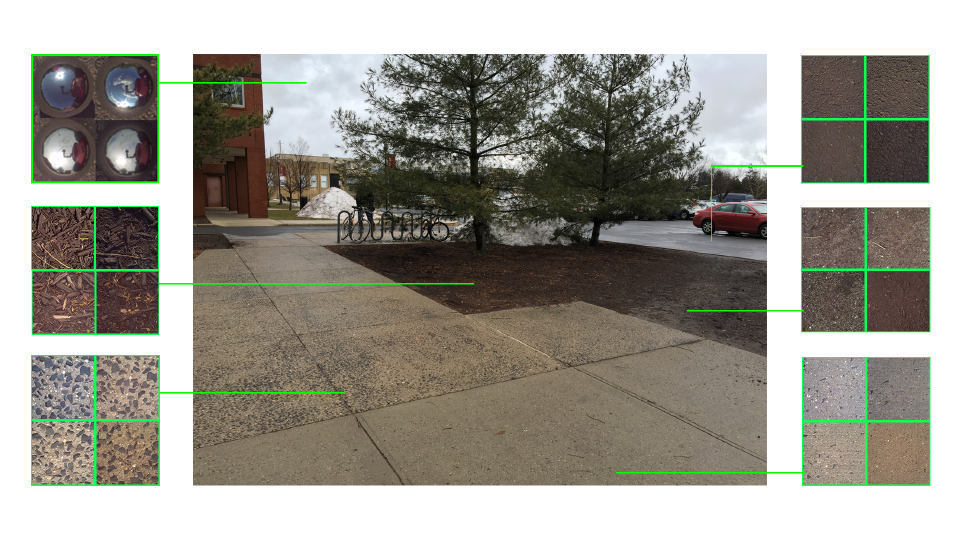
\includegraphics[width=1.0\linewidth]{gtos_dataset.png}
	\caption{Một cảnh ngoài trời được dùng dể lấy các mẫu cho tập dữ liệu GTOS với nhiều góc nhìn nhìn, điều kiện chiếu sáng khác nhau \cite{xue2017differential}}
	\label{fig:gtos_dataset}
\end{figure}

\begin{figure}[h!]
\centering
\captionsetup{width=0.7\textwidth}
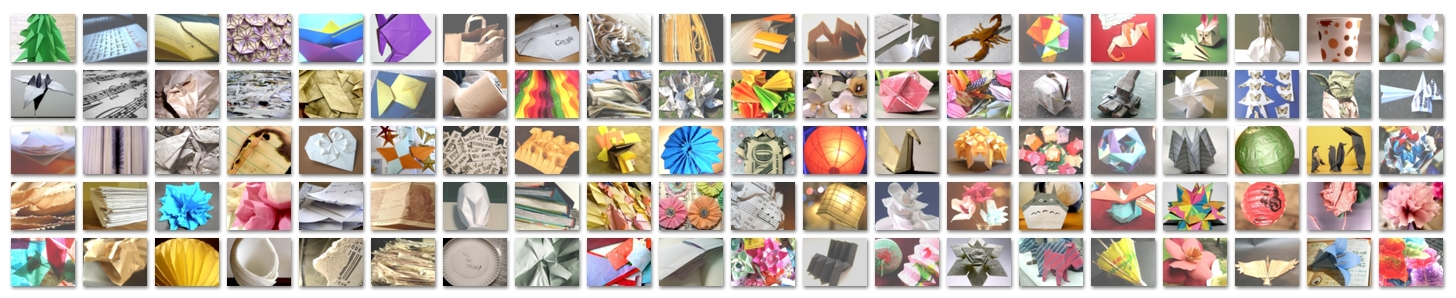
\includegraphics[width=1.0\linewidth]{fmd.png}
\caption{Một tập ảnh từ FMD, đảm bảo sự đa dạng về điều kiện chiếu sáng, bố cục, màu sắc, kết cấu}
\label{fig:fmd}
\end{figure}

\section{Evaluation measures}
Trong cả hai tập dữ liệu, độ chính xác trung bình (mean accuracy) được dùng để đánh giá kết quả cho tất cả các thực nghiệm.

\section{Quá trình thực nghiệm và kết quả}
Nhóm cài đặt các thực nghiệm bằng ngôn ngữ Python với sự hổ trợ của framework scikit-learn và keras (trên nền tensorflow). Mạng VGG16 được huấn luyện sẵn trên ImageNet cũng được dùng cho việc transfer learning và các thực nghiệm khác nhằm hiểu rõ hơn về cách hoạt động của các layer trong CNN.

Tập dữ liệu được chia thành hai tập training và test theo tỷ lệ như các nghiên cứu trước sử dụng: 70\% cho training và 30\% cho test trên tập GTOS, 80\% cho training và 20\% cho test trên tập FMD.

\subsection*{Thực nghiệm với ba mô hình đề xuất}
Đầu tiên nhóm thực hiện rút các handcrafted feature từ ảnh gốc sử dụng các filter thích hợp, bên cạnh đó deep feature cũng được rút từ layer "fc2" của mạng VGG16, sau đó thực hiện huấn luyện các bộ phân lớp ứng với các features khác nhau sử dụng SVMs với nhiều bộ tham số khác nhau, sau cùng dùng các bộ phân lớp này để phân lớp ảnh trên tập test. Probability prediction (trong mô hình 1 và 3) được kết hợp với nhau bằng phép toán trung bình cộng. Và các features được kết hợp với nhau (trong mô hình 2 và 3) bằng phép nối vector (vector concatenation). Các bộ tham số ban đầu (của SVMs) dùng để huấn luyện các bộ phân lớp được ghi nhận lại, từ đó nhóm đánh giá kết quả, điều chỉnh các tham số này thích hợp theo thời gian để có kết quả tốt nhất.

\begin{table}[h!]
  \label{tab:gtos_evaluation}
  \begin{center}
    \resizebox{\linewidth}{!}{
    \begin{tabular}{lccc}
      \toprule[1.0pt]
      \head{Method} 	
      & \head{Deep feature} 
      & \head{Deep+edges} 
      & \head{Deep+edges+textures} \\
      \midrule
      Combine prediction & $75 \pm 1.8$ 	& $75.5 \pm 3.0$  	& $76.3 \pm 1.9$ \\
      Combine features   & $75 \pm 1.8$	& $77.8 \pm 2.5$	& $79.5 \pm 2.5$ \\
      Kết hợp cả hai	   & $75 \pm 1.8$	& $78.9 \pm 2.2$  	& $\textbf{82.2} \pm \textbf{2.3}$\\
      \bottomrule[1.0pt]
    \end{tabular}}
    \captionsetup{width=0.9\textwidth}
    \caption{Kết quả thực nghiệm với các mô hình trên tập GTOS}
  \end{center}
\end{table}

\begin{table}[h!]
  \label{tab:fmd_evaluation}
  \begin{center}
  \resizebox{\linewidth}{!}{
  \begin{tabular}{lccc}
    \toprule[1.0pt]
    \head{Method} 	& \head{Deep feature} 
                    & \head{Deep+edges} 
                    & \head{Deep+edges+textures} \\
    \midrule
    Combine prediction & $74.2 \pm 1.4$ & $75.1 \pm 2.2$  	& $75.5 \pm 2.3$ \\
    Combine features   & $74.2 \pm 1.4$	& $75.3 \pm 1.5$	& $76.3 \pm 1.7$ \\
    Mixed two above    & $74.2 \pm 1.4$	& $75.5 \pm 1.2$  	& $\textbf{77.2} \pm \textbf{0.9}$ \\
    \bottomrule[1.0pt]
  \end{tabular}}
  \captionsetup{width=0.9\textwidth}
  \caption{Kết quả thực nghiệm với các mô hình trên tập FMD}
  \end{center}
\end{table}

Bảng \ref{tab:gtos_evaluation} thể hiện kết quả trên tập GTOS và FMD với ba mô hình đề xuất. Kết quả cho thấy mô hình thứ 3 hoạt động tốt nhất. Hai handcrafted features được dùng thể hiện thông tin về hình dạng và texture hoạt động hiệu quả trên hai tập dữ liệu này. Tuy nhiên, có thể thấy ảnh hưởng của hai features này trên hai tập dữ liệu là khác nhau, trên GTOS hiệu quả của chúng lớn hơn so với trên FMD (đối với cả ba mô hình). Lý do cho điều này được cho là do nhiều ảnh trong FMD là một đối tượng chính nằm trên một background còn GTOS ngược lại, toàn bộ hình đều đồng nhất là một bề mặt duy nhất (Hình \ref{fig:fmd_vs_gtos}). Chính background này khiến thông tin về hình dạng và texture bị ảnh hưởng khác nhiều.

\begin{figure}[h!]
\centering
\captionsetup{width=0.9\textwidth}
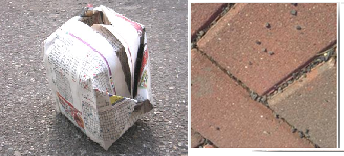
\includegraphics[width=0.75\linewidth]{fmd_vsgtos.png}
\caption{Ảnh từ FMD (bên trái) trong lớp vật liệu "giấy" lại có background là một mặt đường khiến thông tin về texture không còn sự hiệu quả, trong khi ảnh từ GTOS là một bề mặt đồng nhất duy nhất (lớp "Gạch")}
\label{fig:fmd_vs_gtos}
\end{figure}

\begin{table}
\label{tab:comparasion}
\begin{center}
\resizebox{0.6\linewidth}{!}{
\begin{tabular}{lccc}
\toprule[1.0pt]
\head{Method}
				& \head{GTOS} 
                & \head{FMD} \\
\midrule
DAIN & $81.2 \pm 1.7$ & \\
Reflectance  & & $65.5$ \\
SIFT IFV+fc7 & & $69.6 \pm 0.3$ \\
Ours    & $\textbf{82.2}$ & $\textbf{77.2}$ \\
\bottomrule[1.0pt]
\end{tabular}}
\captionsetup{width=0.45\textwidth}
\caption{So sánh kết quả với các phương pháp khác trên 
GTOS và FMD \cite{xue2017differential} \cite{zhang2015reflectance}} \cite{bell2015material}
\end{center}
\end{table}

\begin{figure}[h!]
\centering
\captionsetup{width=0.45\textwidth}
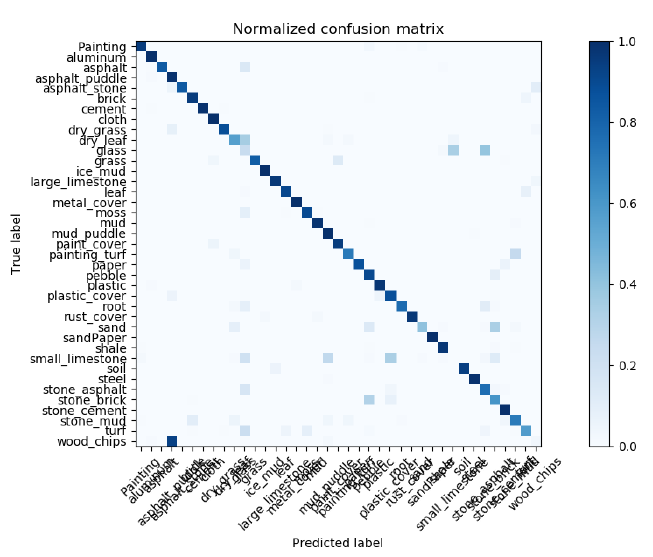
\includegraphics[width=0.9\linewidth]{gtos_confusion.png}
\caption{Normalized confusion matrix trên GTOS}
\label{fig:gtos_confusion}
\end{figure}

\begin{figure}[h!]
\centering
\captionsetup{width=0.45\textwidth}
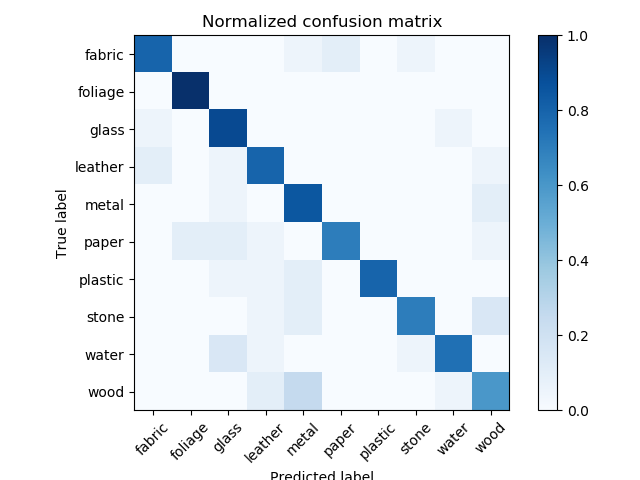
\includegraphics[width=0.9\linewidth]{fmd_confusion.png}
\caption{Normalized confusion matrix trên FMD}
\label{fig:gtos_confusion}
\end{figure}

\begin{table}[h!]
  \label{tab:comparasion}
  \begin{center}
    \resizebox{1.0\linewidth}{!}{
    \begin{tabular}{lr|lr|lr|lr}
      \toprule[1.0pt]
      \head{Classes}
      & \head{Acc.}
      & \head{Classes}
      & \head{Acc.}
      & \head{Classes}
      & \head{Acc.}
      & \head{Classes}
      & \head{Acc.} \\
      \midrule
      painting 		& 0.95 & glass 				& 0.83 & painting turf 	& 0.96 & small limestone 	& 0.87	\\
      aluminum 		& 0.82 & grass 				& 0.98 & paper 			& 0.90 & soil 				& 0.77	\\
      asphalt 		& 0.90 & ice mud 			& 0.84 & pebble			& 0.91 & steel				& 0.96	\\
      asphalt puddle 	& 0.76 & large limestone 	& 0.95 & plastic		& 0.89 & stone asphalt		& 0.40	\\
      asphalt stone 	& 0.60 & leaf 				& 0.99 & plastic cover	& 0.98 & stone brick		& 0.92	\\
      brick 			& 0.99 & metal cover 		& 0.92 & root			& 0.99 & stone cement		& 0.97	\\
      cement 			& 0.71 & moss 				& 0.88 & rust cover		& 0.94 & stone mud			& 0.97	\\
      cloth 			& 0.57 & mud 				& 0.56 & sand			& 0.71 & turf				& 0.94	\\
      dry grass 		& 0.93 & mud puddle			& 0.23 & sand paper		& 0.87 & wood chips			& 0.98	\\
      dry leaf 		& 0.95 & paint cover 		& 0.85 & shale			& 0.97 & 					&		\\
      \bottomrule[1.0pt]
    \end{tabular}}
    \captionsetup{width=0.9\textwidth}
    \caption{Kết quả cho từng lớp vật liệu trên tập GTOS}
  \end{center}
\end{table}

\subsection*{Thực nghiệm với VGG16 (nền tảng để xây dựng một CNN mới)}

\begin{figure}[h!]
\centering
\captionsetup{width=0.9\textwidth}
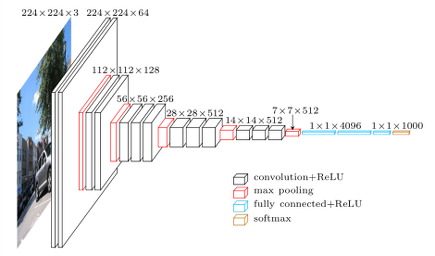
\includegraphics[width=1.0\linewidth]{vgg16.png}
\caption{Cấu trục mạng VGG16 được nhóm dùng để rút trích đặc trưng ở layer 'fc2' và thực hiện các thực nghiệm ở phần thực nghiệm với VGG16}
\label{fig:vgg16}
\end{figure}

Quá trình thực nghiệm với VGG16 qua các bước sau đây:
\begin{enumerate}
\item Fine-tune VGG16: Thay fully-connected layer cuối cùng để đầu ra là 39 lớp (trên GTOS) thay vì 1000 lớp (trên ImageNet) và huấn luyện lại giá trị tham số của layer này, sau đó huấn luyện lại tất cả các layer để so sánh kết quả.
\item Tìm hiểu sự ảnh hưởng của các layer trong mạng bằng cách bỏ bớt layer trong mạng, quan sát ảnh hưởng của các layer này trên kết quả thu được.
\item QUa quan sát từ bước 2 và dựa trên nền của VGG16 chọn các layer thích hợp để xây dựng một mạng CNN ít layer hơn nhưng đạt kết quả xấp xĩ.
\end{enumerate}

Hiện tại, khi đang viết luận văn này, nhóm vẫn đang thực nghiệm ở bước một, kết quả sau khi fine-tune trên GTOS cho thấy thời gian giảm 1/3 so với sử dụng SVM (bao gồm thời gian rút trích đặc trưng, huấn luyện và test), không cần tốn không gian lưu trữ đặc trưng và độ chính xác giảm từ $82.2\%$ xuống còn $79.8\%$.
